\documentclass[journal]{vgtc}                % final (journal style)
%\documentclass[review,journal]{vgtc}         % review (journal style)
%\documentclass[widereview]{vgtc}             % wide-spaced review
%\documentclass[preprint,journal]{vgtc}       % preprint (journal style)
%\documentclass[electronic,journal]{vgtc}     % electronic version, journal

%% Uncomment one of the lines above depending on where your paper is
%% in the conference process. ``review'' and ``widereview'' are for review
%% submission, ``preprint'' is for pre-publication, and the final version
%% doesn't use a specific qualifier. Further, ``electronic'' includes
%% hyperreferences for more convenient online viewing.

%% Please use one of the ``review'' options in combination with the
%% assigned online id (see below) ONLY if your paper uses a double blind
%% review process. Some conferences, like IEEE Vis and InfoVis, have NOT
%% in the past.

%% Please note that the use of figures other than the optional teaser is not permitted on the first page
%% of the journal version.  Figures should begin on the second page and be
%% in CMYK or Grey scale format, otherwise, colour shifting may occur
%% during the printing process.  Papers submitted with figures other than the optional teaser on the
%% first page will be refused.

%% These three lines bring in essential packages: ``mathptmx'' for Type 1
%% typefaces, ``graphicx'' for inclusion of EPS figures. and ``times''
%% for proper handling of the times font family.

\usepackage{mathptmx}
\usepackage{graphicx}
\usepackage{times}

%% We encourage the use of mathptmx for consistent usage of times font
%% throughout the proceedings. However, if you encounter conflicts
%% with other math-related packages, you may want to disable it.

%% This turns references into clickable hyperlinks.
\usepackage[bookmarks,backref=true,linkcolor=black]{hyperref} %,colorlinks
\hypersetup{
  pdfauthor = {},
  pdftitle = {},
  pdfsubject = {},
  pdfkeywords = {},
  colorlinks=true,
  linkcolor= black,
  citecolor= black,
  pageanchor=true,
  urlcolor = black,
  plainpages = false,
  linktocpage
}

%% If you are submitting a paper to a conference for review with a double
%% blind reviewing process, please replace the value ``0'' below with your
%% OnlineID. Otherwise, you may safely leave it at ``0''.
\onlineid{0}

%% declare the category of your paper, only shown in review mode


%% allow for this line if you want the electronic option to work properly


%% In preprint mode you may define your own headline.
%\preprinttext{To appear in an IEEE VGTC sponsored conference.}

%% Paper title.

\title{Visual Analytics on Credit Cards Defaults}
%\subtitle{Visual Analytics project, A.Y. 2017/2018}

%% This is how authors are specified in the journal style

%% indicate IEEE Member or Student Member in form indicated below
\author{Maria Ludovica Costagliola, Emanuele De Santis}


%other entries to be set up for journal
%\shortauthortitle{Firstauthor \MakeLowercase{\textit{et al.}}: Paper Title}

%% Abstract section.
\abstract{
The project was developed during the Visual Analytics course. It concerns the visualization of credit cards owners data in order to
make the bank director knowing the customers that are supposed to not be able to pay the credit card bill in the next month.

All data are represented using simple and well-known views that immediately highlights similarities among customers and give to the user an
overview on all customers.

The system uses also a machine learning algorithm to classify new customers (manually added using a form) and represents them updating the views.

} % end of abstract

%% Keywords that describe your work. Will show as 'Index Terms' in journal
%% please capitalize first letter and insert punctuation after last keyword


%% ACM Computing Classification System (CCS).
%% See <http://www.acm.org/class/1998/> for details.
%% The ``\CCScat'' command takes four arguments.


%% Uncomment below to include a teaser figure.
  \teaser{
 \centering
 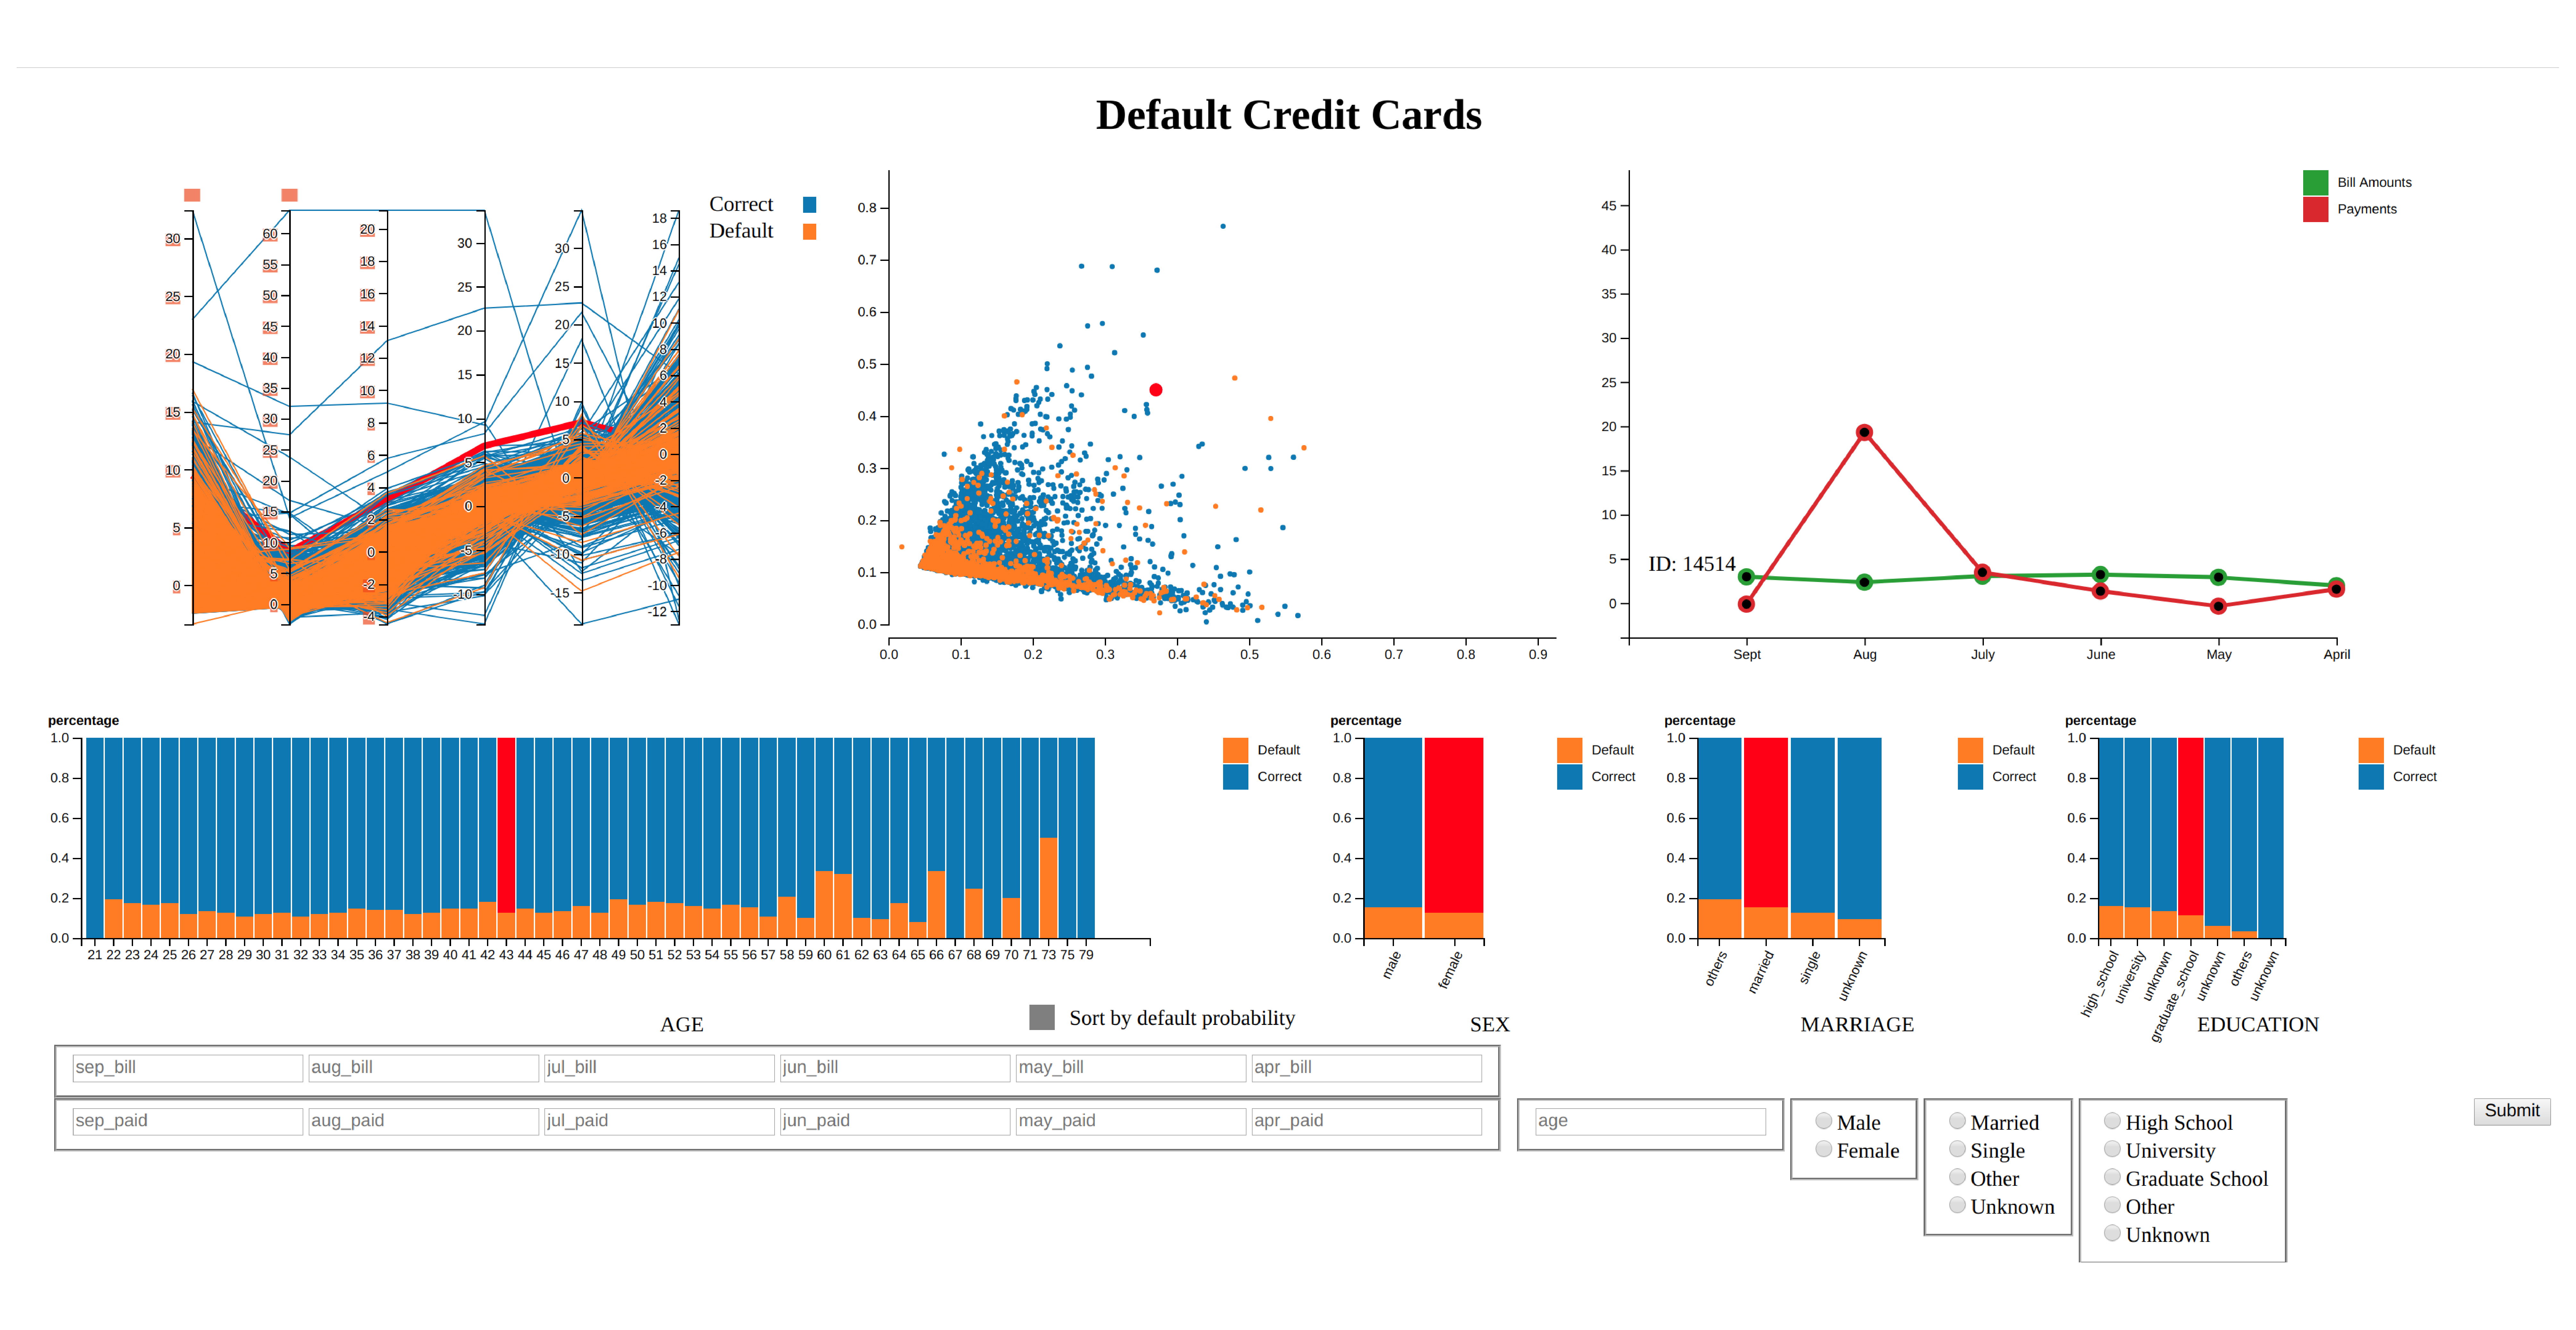
\includegraphics[width=16cm]{views}
  \caption{Sceenshot of the entire interface}
  }

%% Uncomment below to disable the manuscript note
\renewcommand{\manuscriptnotetxt}{}

%% Copyright space is enabled by default as required by guidelines.
%% It is disabled by the 'review' option or via the following command:
% \nocopyrightspace

%%%%%%%%%%%%%%%%%%%%%%%%%%%%%%%%%%%%%%%%%%%%%%%%%%%%%%%%%%%%%%%%
%%%%%%%%%%%%%%%%%%%%%% START OF THE PAPER %%%%%%%%%%%%%%%%%%%%%%
%%%%%%%%%%%%%%%%%%%%%%%%%%%%%%%%%%%%%%%%%%%%%%%%%%%%%%%%%%%%%%%%%

\begin{document}

%% The ``\maketitle'' command must be the first command after the
%% ``\begin{document}'' command. It prepares and prints the title block.

%% the only exception to this rule is the \firstsection command
\firstsection{Introduction}

\maketitle

%% \section{Introduction} %for journal use above \firstsection{..} instead

After the paper presentation done during the lectures, we decided to focus our attention on a dataset related to bank transactions.
Most of the bank transactions datasets are not public available (or they contains few useful information to protect users' privacy), but we were able to find
a dataset related to this field.

We were thinking about the need for a bank director to always know how customers with a credit card issued by his financial institution behave. Particularly, we pay attention
to the last payments and to the corresponding bank account balances of those customers.

From these data and from some other personal information of the customer (for example age, marriage status, ...), it is possible to identify the ones that probably will not be able
to pay the credit card bill in the next month.

The prediction is done by a machine learning algorithm, but the result is useless if it is not combined with an efficient visualization of the whole data. In fact, with this visualization
a bank director is able to better understand the result of the machine learning algorithm, considering also the similarity between the result and some preexisting patterns or clusters.

Moreover the bank director may be able to detect default customers even without using any machine learning algorithm, just seeing the information given by the visualization.


\section{Dataset}
The dataset used in this project is taken from UCI database \cite{UCI:2016} , it contains about 30000 tuples, each with 24 attributes.
Some tuples lack of some values and so they were all removed in order to have a completely useful dataset. A few attributes for each remaining tuple were also removed because they were of no interest for us. We get in this way a more manageable dataset thanks to a lower number of tuples (15337) and of attributes (19).
This computation was done by the python function \texttt{preprocessing.action()}, that creates a new csv file named \texttt{dataset.csv}.

About the used attributes, we can identify four of them that are categorical: age, sex, marriage status, education. These represent personal information about the owner of a particular credit card and they are used for statistical considerations. We have six numerical attributes named \textit{Amount of bill statement}, one for each month from September 2005 to April 2005 and the corresponding six numerical, named \textit{Amount of previous payment}.

The last attribute of each row is the \textit{target}, that is the prediction about the ability to pay on October 2005.


\section{Visualization}
The visualization that we have developed is constituted by 7 views, each one that shows different aspects of the dataset. All the view are coordinated each other, so clicking on
an element of a certain view will highlight some elements in the other views and/or will show other information. Moreover when a new customer is added, all the views change according to
the newly added tuple.

The interface was tought to fit in a FullHD (1920x1080) screen, even if it works also if we resize the browser window (the minimun resolution supported is 1024x768).


\subsection{Scatterplot}

\begin{figure}
  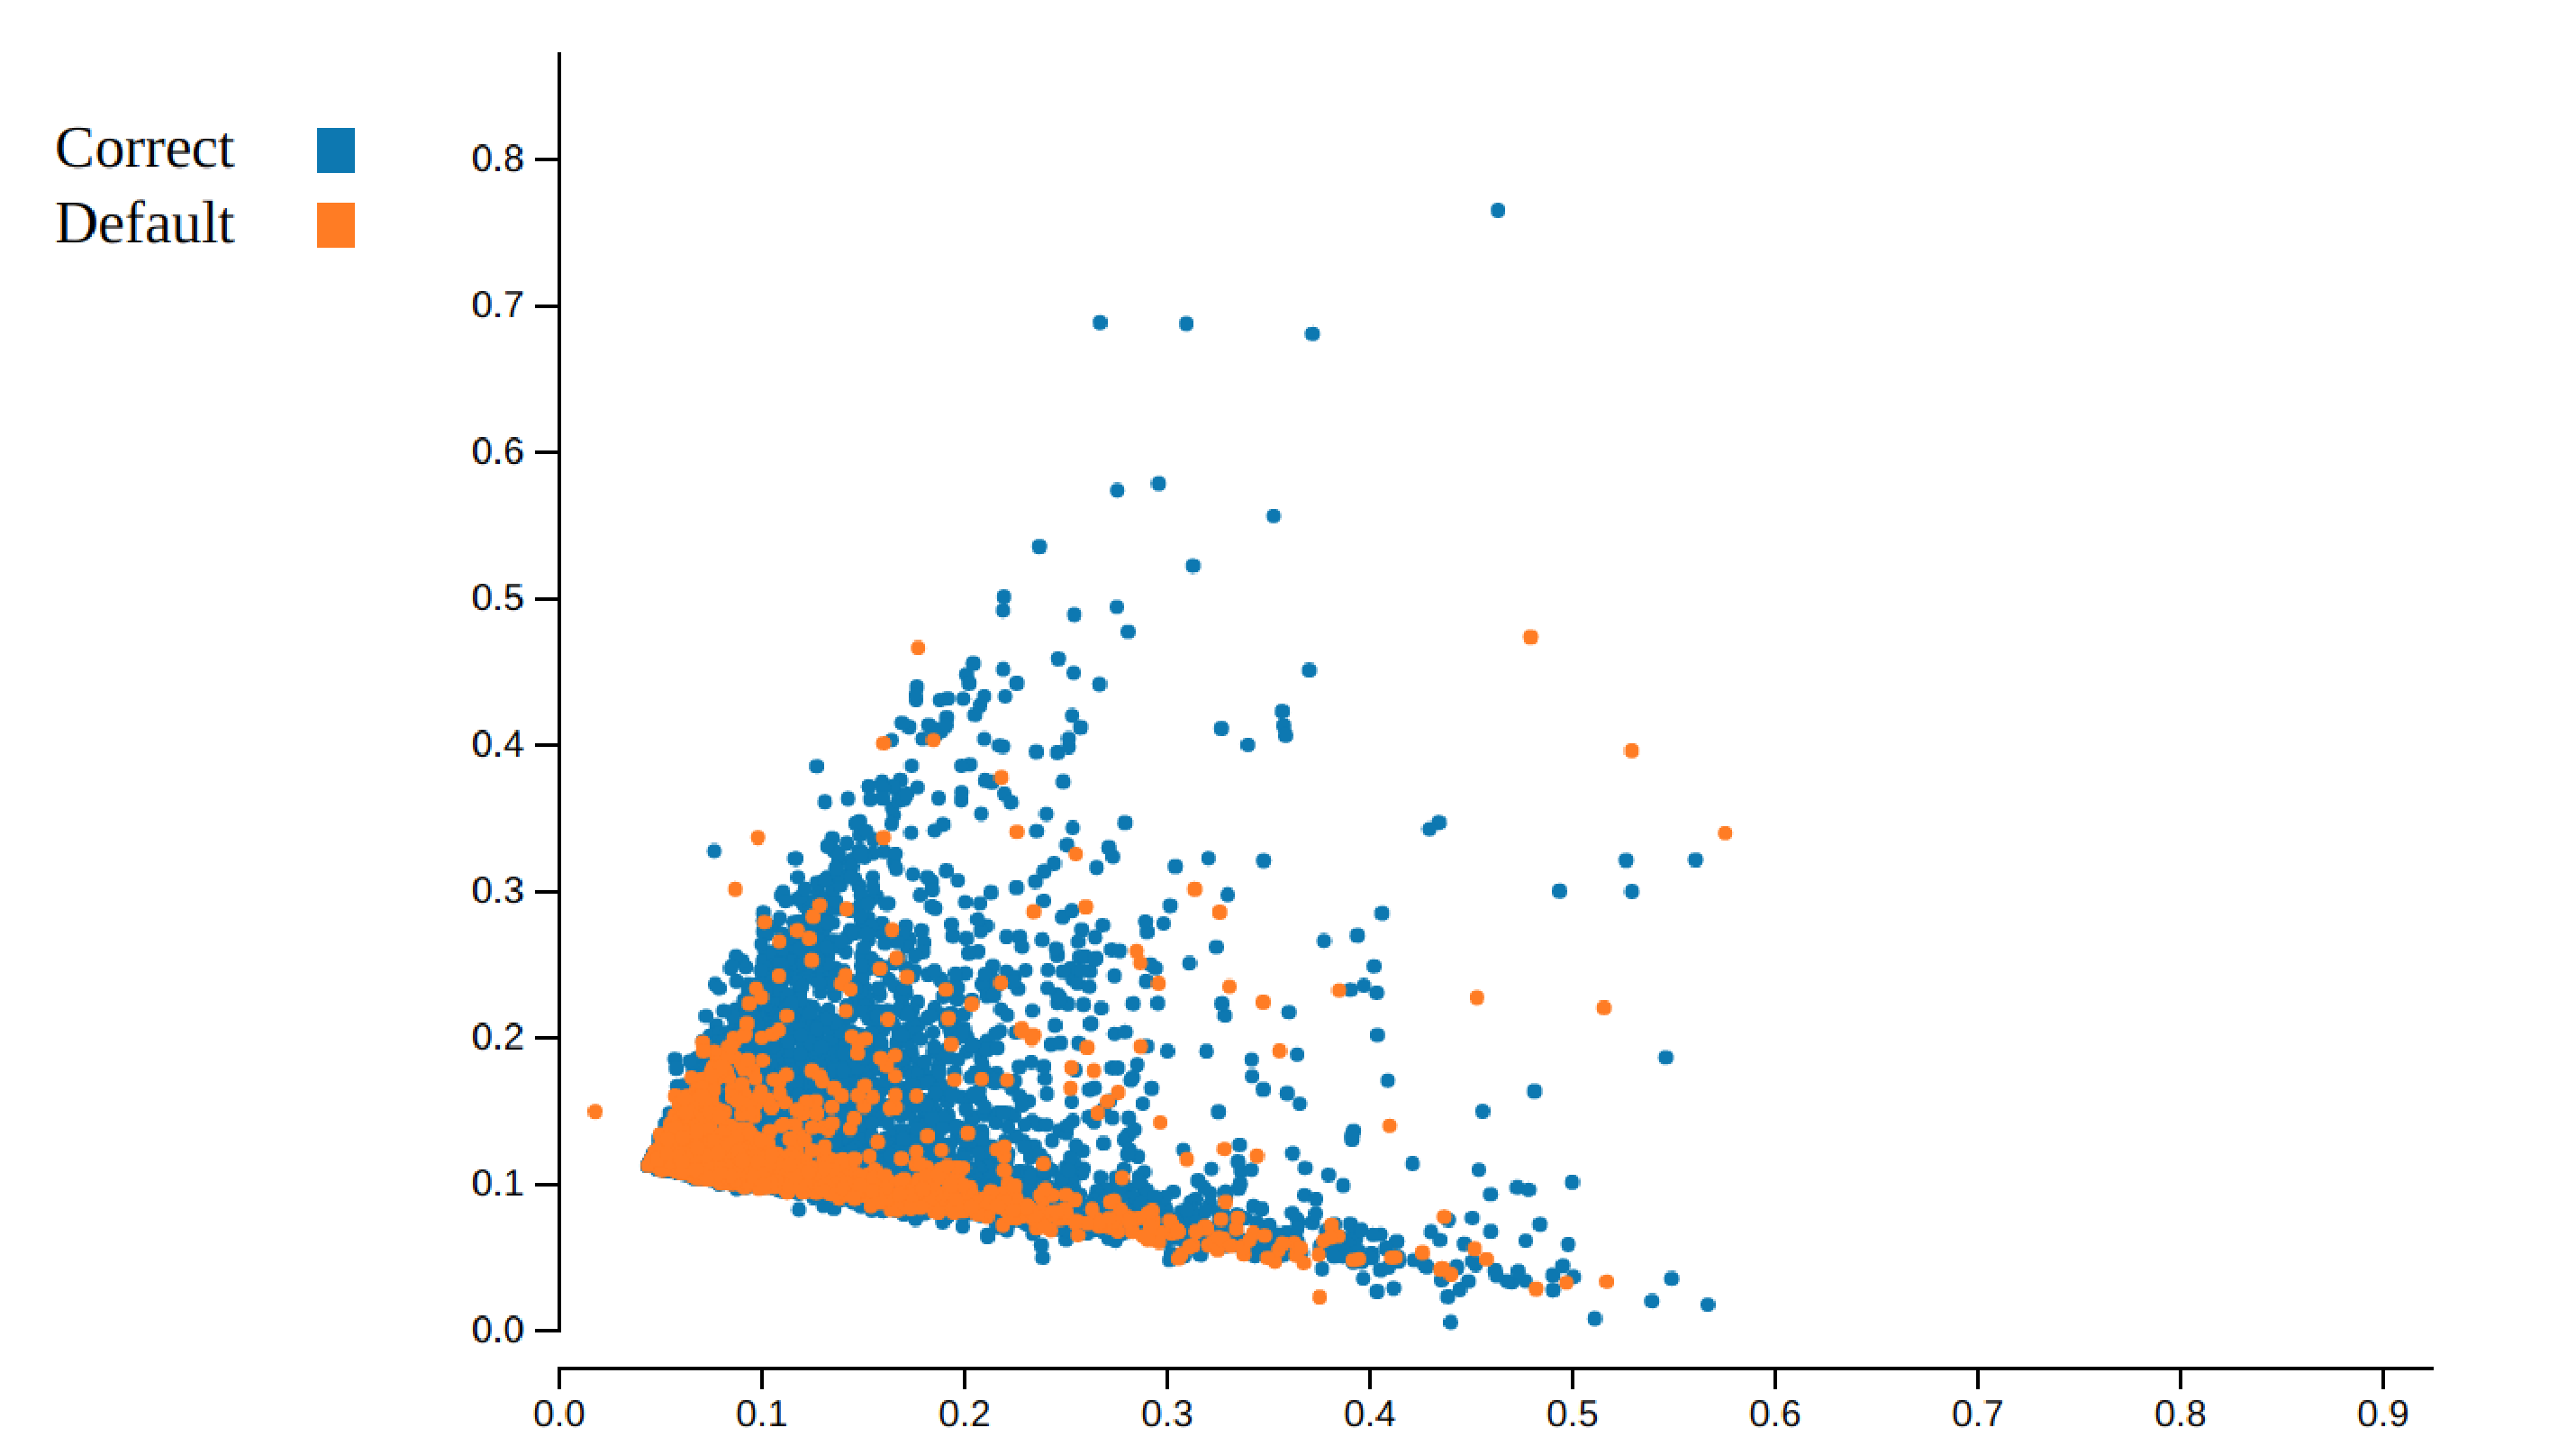
\includegraphics[scale=0.15]{scatterplot}
  \caption{Scatterplot view of the tool}
  \label{scatterplot}
\end{figure}
The scatterplot is the main view in the visualization. Each point represents a customer and the color encodes the classification of the customer (default or correct). The color scaling used is the \texttt{d3.scaleOrdinal(d3.schemeCategory10)}.

Due to the high dimensionality of the dataset, it was mandatory to apply a dimensionality reduction algorithm. We decided to apply PCA because it is fast and it doesn't require a deep knowledge of the problem, and we then took the first 2 components. This work is done by the python function \texttt{pca.action()} using \texttt{pandas} to read and parse the csv original dataset
and \texttt{sklearn} to compute PCA values. The result is saved in \texttt{pca.csv}.
A 2D scatterplot is the best way to graphically represent the relation between points and to spot possible clusters. In this case it helps the bank director to quickly see that most of the bad customers are grouped togheter in a particular area (in figure \ref{scatterplot} in the left-bottom part of the plot).

Each point has associated two event handlers. The first one allows to make visible a tooltip showing the identifier of the customer just by mouseovering over it; this handler also makes the point bigger to have it more visible.
The second handler is associated to click events: by clicking on a point, it will highlight the point itself, will trigger the highlighting of the other related elements and will show up the corresponding lines in the linechart.

\subsection{Parallel Coordinates}
The first view that can be seen in the interface is the parallel coordinates chart. We have six axis, that correspond to the first
six principal components given by the PCA algorithm applied on the original dataset. Each line referrs to one single point that is the
graphic representation of a customer. Since each customer can have the target attribute equal to either 0 or 1, we have decided to use two colors to distinguish
among default and correct users.


\section{Conclusion}


%% if specified like this the section will be committed in review mode
\acknowledgments{
}

\bibliographystyle{abbrv}
%%use following if all content of bibtex file should be shown
%\nocite{*}
\bibliography{template}
\end{document}
